\documentclass{article}
\usepackage[margin=2cm]{geometry}
\usepackage{graphicx}
\usepackage{subcaption}
\usepackage{tabu}
\usepackage{mathtools}
%\usepackage{amsmath}
% \graphicspath{ {Q1/images/}{Q2/images/}{Q3/images/}{Q4/images/} }
\title{COL783 Assignment 1}
\date{}
\author{Lovish Madaan \\ \texttt{2015CS50286} \and Nikhil Goyal \\ \texttt{2015CS50287}}
\begin{document}
\maketitle
\section{Color Quantization}

% \begin{figure}[!ht]
% \centering
% 
\includegraphics[scale=0.7]{img1_1.png}
% \caption{Plot of the training data along with the learned linear hypothesis}
% \end{figure}

\begin{figure}[!ht]
\begin{subfigure}{.5\textwidth}
\centering
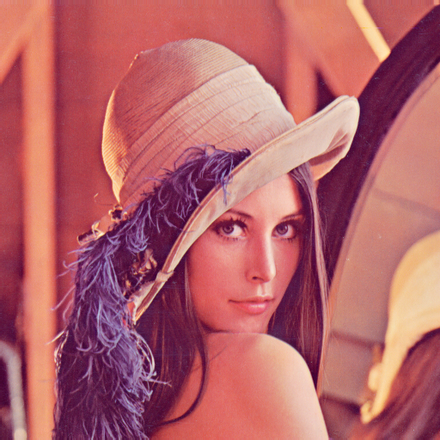
\includegraphics[width=.75\linewidth]{lenna.png}
\caption{Original Image}
\end{subfigure}
\begin{subfigure}{.5\textwidth}
\centering

\includegraphics[width=.75\linewidth]{img1_1.png}
\caption{Popularity Algorithm with $n = 4$}
\end{subfigure}
\end{figure}

\begin{figure}[!ht]
\begin{subfigure}{.5\textwidth}
\centering

\includegraphics[width=.75\linewidth]{img1_2.png}
\caption{Median Cut with $n = 4$}
\end{subfigure}
\begin{subfigure}{.5\textwidth}
\centering
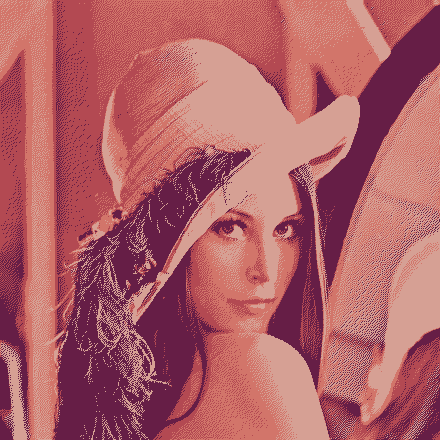
\includegraphics[width=.75\linewidth]{img1_3.png}
\caption{Median Cut($n = 4$) with dithering}
\end{subfigure}
\end{figure}

\clearpage

\begin{figure}[!ht]
\begin{subfigure}{.5\textwidth}
\centering
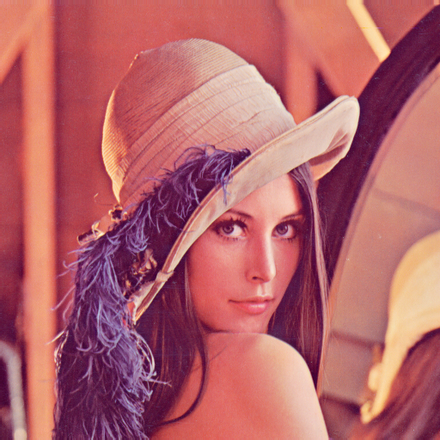
\includegraphics[width=.75\linewidth]{lenna.png}
\caption{Original Image}
\end{subfigure}
\begin{subfigure}{.5\textwidth}
\centering
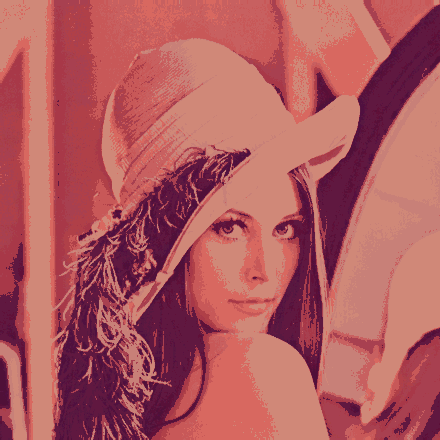
\includegraphics[width=.75\linewidth]{img1_1_16.png}
\caption{Popularity Algorithm with $n = 16$}
\end{subfigure}
\end{figure}

\begin{figure}[!ht]
\begin{subfigure}{.5\textwidth}
\centering
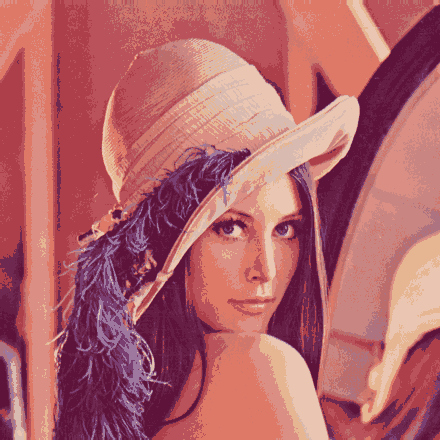
\includegraphics[width=.75\linewidth]{img1_2_16.png}
\caption{Median Cut with $n = 16$}
\end{subfigure}
\begin{subfigure}{.5\textwidth}
\centering
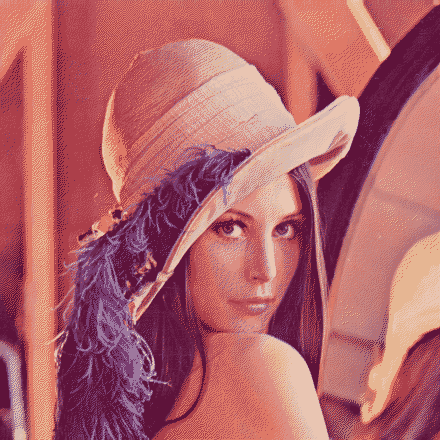
\includegraphics[width=.75\linewidth]{img1_3_16.png}
\caption{Median Cut($n = 16$) with dithering}
\end{subfigure}
\end{figure}

\clearpage

\section{Edge Detection}

\subsection{Tanh Toning Function}

\begin{figure}[!ht]
\begin{subfigure}{.5\textwidth}
\centering
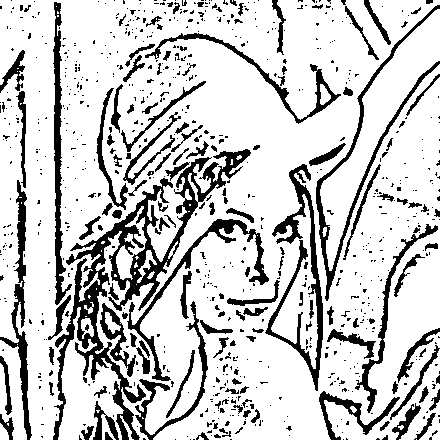
\includegraphics[width=.75\linewidth]{xdog4.png}
\caption{Edge Detection using xDoG, $n = 4$}
\end{subfigure}
\begin{subfigure}{.5\textwidth}
\centering
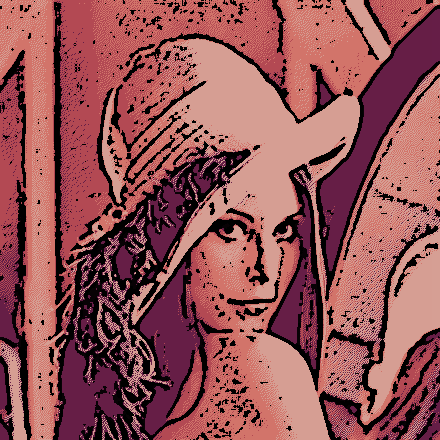
\includegraphics[width=.75\linewidth]{pastel4.png}
\caption{Painterly Output, $n = 4$}
\end{subfigure}
\end{figure}

\begin{figure}[!ht]
\begin{subfigure}{.5\textwidth}
\centering
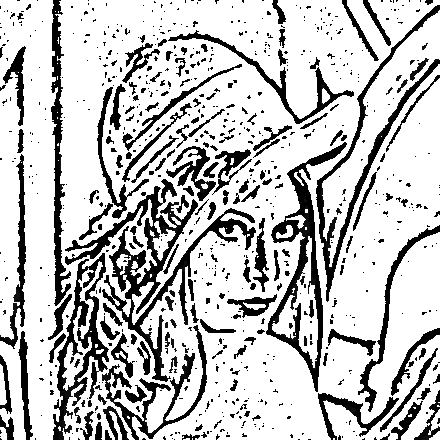
\includegraphics[width=.75\linewidth]{xdog16.png}
\caption{Edge Detection using xDoG, $n = 16$}
\end{subfigure}
\begin{subfigure}{.5\textwidth}
\centering
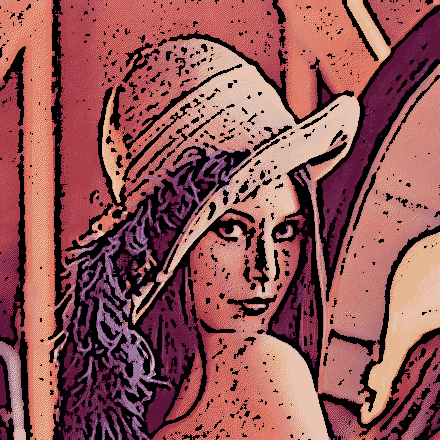
\includegraphics[width=.75\linewidth]{pastel16.png}
\caption{Painterly Output, $n = 16$}
\end{subfigure}
\end{figure}

\clearpage

\subsection{Sigmoid Toning Function}

\begin{figure}[!ht]
\begin{subfigure}{.5\textwidth}
\centering
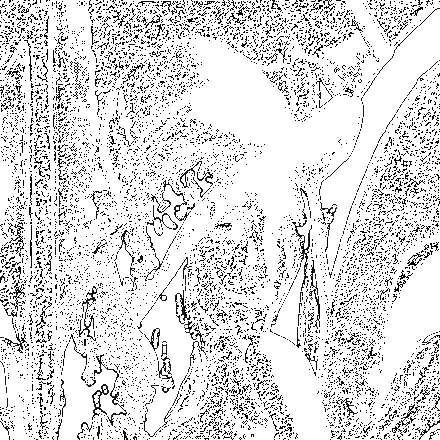
\includegraphics[width=.75\linewidth]{xdogsig4.png}
\caption{Edge Detection using xDoG, $n = 4$}
\end{subfigure}
\begin{subfigure}{.5\textwidth}
\centering
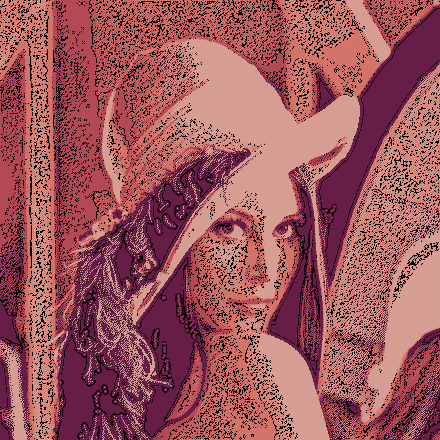
\includegraphics[width=.75\linewidth]{pastelsig4.png}
\caption{Painterly Output, $n = 4$}
\end{subfigure}
\end{figure}

\begin{figure}[!ht]
\begin{subfigure}{.5\textwidth}
\centering
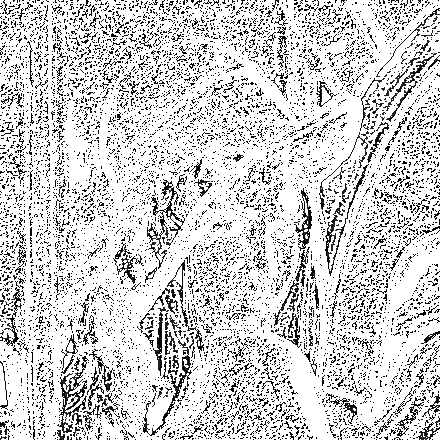
\includegraphics[width=.75\linewidth]{xdogsig16.png}
\caption{Edge Detection using xDoG, $n = 16$}
\end{subfigure}
\begin{subfigure}{.5\textwidth}
\centering
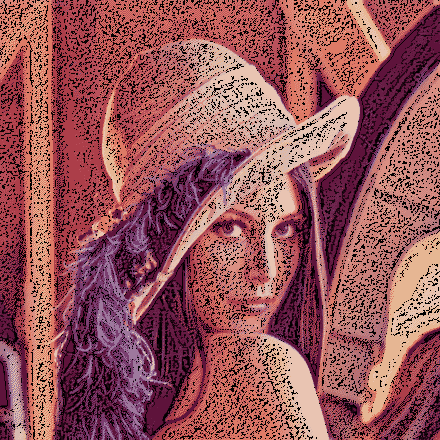
\includegraphics[width=.75\linewidth]{pastelsig16.png}
\caption{Painterly Output, $n = 16$}
\end{subfigure}
\end{figure}

\end{document}